\documentclass[aspectratio=169]{beamer}

%=========================================================
% Packages
%=========================================================

\usetheme{Madrid}

\usepackage[T1]{fontenc}
\usepackage{lmodern}

\usepackage{graphicx}
\usepackage{booktabs}
\usepackage{tikz}
\usetikzlibrary{positioning,arrows.meta,shapes.geometric}

\usepackage{hyperref}

%=========================================================
% Colors
%=========================================================

\definecolor{CNUBlue}{RGB}{0,51,102}
\definecolor{CNUGold}{RGB}{181,136,52}

\setbeamercolor{structure}{fg=CNUBlue}
\setbeamercolor{title}{fg=white,bg=CNUBlue}
\setbeamercolor{frametitle}{fg=white,bg=CNUBlue}

%=========================================================
% Title Information
%=========================================================

\title{Building an Explainable Institutional Reasoning System}
\subtitle{A Prototype for Strategic Academic Decision Support}

\author{Edward Brash}

\institute{
School of Engineering and Computing\\
Christopher Newport University
}

\date{July 2026}

%=========================================================
% Document
%=========================================================

\begin{document}

%=========================================================
\begin{frame}
    \titlepage
\end{frame}

%=========================================================
\begin{frame}{Motivation}

\Large

Our original discussion began with a simple question:

\vspace{0.8cm}

\begin{block}{Question}
Can artificial intelligence become an active participant in
strategic academic planning while remaining transparent,
explainable, and defensible?
\end{block}

\vspace{0.8cm}

This project explores one possible answer.

\end{frame}

%=========================================================
\begin{frame}{The Challenge}

Universities routinely make strategic decisions involving

\vspace{0.25cm}

\begin{itemize}
\item enrollment trends
\item academic program development
\item faculty hiring
\item accreditation
\item budgeting
\item long-term strategic planning
\end{itemize}

\vspace{0.35cm}

\begin{block}{How these decisions are often made}
They rely heavily upon collective human knowledge accumulated
over many years---what we call \textbf{institutional memory}.
\end{block}

\vspace{0.25cm}

That memory is enormously valuable, but it is difficult to preserve,
search, update, and transfer.

\end{frame}

%=========================================================
\begin{frame}{Traditional Decision Support}

\begin{columns}[T]

\column{0.48\textwidth}

\begin{block}{Institutional Memory}

\begin{itemize}
\item Experienced administrators
\item Experienced faculty and staff
\item Committee deliberation
\item Historical knowledge
\item Informal relationships
\end{itemize}

\end{block}

\column{0.48\textwidth}

\begin{block}{Supporting Materials}

\begin{itemize}
\item Reports
\item Spreadsheets
\item Policies
\item Accreditation records
\item Planning documents
\end{itemize}

\end{block}

\end{columns}

\vspace{0.4cm}

The institution possesses substantial knowledge, but much of it is
distributed across people, files, systems, and historical records.

\vspace{0.25cm}

Every new question can therefore require reconstructing the relevant
institutional context.

\end{frame}

%=========================================================
\begin{frame}{A Different Vision}

\Large

Rather than producing another report...

\vspace{0.8cm}

\begin{center}

{\Huge Build an Institutional Reasoning System}

\end{center}

\vspace{0.8cm}

that continuously

\begin{itemize}
\item organizes institutional knowledge,
\item retrieves relevant evidence,
\item evaluates scenarios,
\item produces explainable recommendations,
\item and supports---rather than replaces---human judgment.
\end{itemize}

\end{frame}

%=========================================================
\begin{frame}{Guiding Principles}

\begin{block}{Design Philosophy}

The objective is \textbf{not} automated decision making.

\vspace{0.3cm}

The objective is to augment human decision making with
transparent, evidence-based reasoning.

\end{block}

\vspace{0.5cm}

Every recommendation should be

\begin{itemize}

\item Explainable

\item Defensible

\item Traceable to institutional evidence

\item Reproducible

\item Open to human review

\end{itemize}

\end{frame}

%=========================================================
\begin{frame}{Prototype Architecture}

\centering

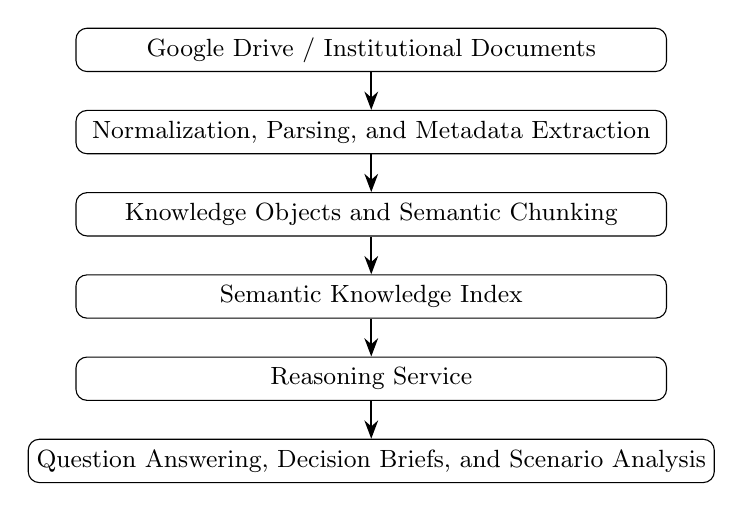
\begin{tikzpicture}[
node distance=0.48cm,
every node/.style={
    draw,
    rounded corners,
    minimum width=7.5cm,
    minimum height=0.55cm,
    inner sep=3pt,
    align=center,
    font=\small
},
>=Stealth
]

\node (drive) {Google Drive / Institutional Documents};

\node (norm) [below=of drive]
{Normalization, Parsing, and Metadata Extraction};

\node (chunks) [below=of norm]
{Knowledge Objects and Semantic Chunking};

\node (index) [below=of chunks]
{Semantic Knowledge Index};

\node (reason) [below=of index]
{Reasoning Service};

\node (brief) [below=of reason]
{Question Answering, Decision Briefs, and Scenario Analysis};

\draw[->,thick] (drive)--(norm);
\draw[->,thick] (norm)--(chunks);
\draw[->,thick] (chunks)--(index);
\draw[->,thick] (index)--(reason);
\draw[->,thick] (reason)--(brief);

\end{tikzpicture}

\end{frame}
%=========================================================
\begin{frame}{From Documents to Institutional Knowledge}

\centering

\vspace{0.55cm}

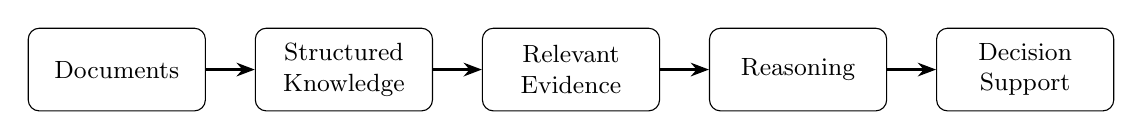
\begin{tikzpicture}[
node distance=0.62cm,
every node/.style={
    draw,
    rounded corners,
    minimum width=2.25cm,
    minimum height=1.05cm,
    inner sep=4pt,
    align=center,
    font=\small
},
>=Stealth
]

\node (documents) {Documents};

\node (knowledge) [right=of documents]
{Structured\\Knowledge};

\node (evidence) [right=of knowledge]
{Relevant\\Evidence};

\node (reasoning) [right=of evidence]
{Reasoning};

\node (support) [right=of reasoning]
{Decision\\Support};

\draw[->,thick] (documents)--(knowledge);
\draw[->,thick] (knowledge)--(evidence);
\draw[->,thick] (evidence)--(reasoning);
\draw[->,thick] (reasoning)--(support);

\end{tikzpicture}

\vspace{0.95cm}

The system does not ask a language model to read every institutional
document for every question.

\vspace{0.35cm}

It first identifies the small body of evidence most relevant to the
specific decision, and then asks the reasoning service to analyze it.

\end{frame}

%=========================================================
\begin{frame}{An Important Architectural Principle}

\small

\begin{block}{Knowledge objects store facts.}

Documents, metadata, source locations, semantic chunks,
timestamps, and provenance.

\end{block}

\vspace{0.25cm}

\begin{block}{Services derive meaning.}

Retrieval, ranking, synthesis, scenario evaluation,
decision support, and institutional reasoning.

\end{block}

\vspace{0.35cm}

\begin{center}
\large
\textbf{Knowledge objects store facts. Services derive meaning.}
\end{center}

\vspace{0.25cm}

This separation allows the same institutional knowledge layer to
support multiple applications without embedding conclusions or
recommendations permanently into the underlying data.

\end{frame}

%=========================================================
\begin{frame}{Why Explainability Matters}

Traditional AI systems often produce answers without showing
how they were obtained.

\vspace{0.4cm}

For institutional decision support, that is unacceptable.

\vspace{0.5cm}

Every recommendation should answer three questions:

\begin{enumerate}

\item What evidence was used?

\vspace{0.2cm}

\item Why was that evidence selected?

\vspace{0.2cm}

\item Could another person independently reproduce the result?

\end{enumerate}

\vspace{0.6cm}

Our architecture was designed around these questions from the
very beginning.

\end{frame}

%=========================================================
\begin{frame}{The Semantic Observatory}

\begin{columns}

\column{0.50\textwidth}

The prototype continuously monitors the health of the semantic
ecosystem.

\vspace{0.4cm}

Examples include

\begin{itemize}

\item document counts

\item parser statistics

\item chunk distributions

\item corpus dominance

\item outlier detection

\item parser quality

\item retrieval benchmarking

\end{itemize}

\column{0.5\textwidth}

\centering

\fbox{
\parbox[c][6.8cm][c]{0.95\linewidth}{
\vspace{2.3cm}

\begin{center}
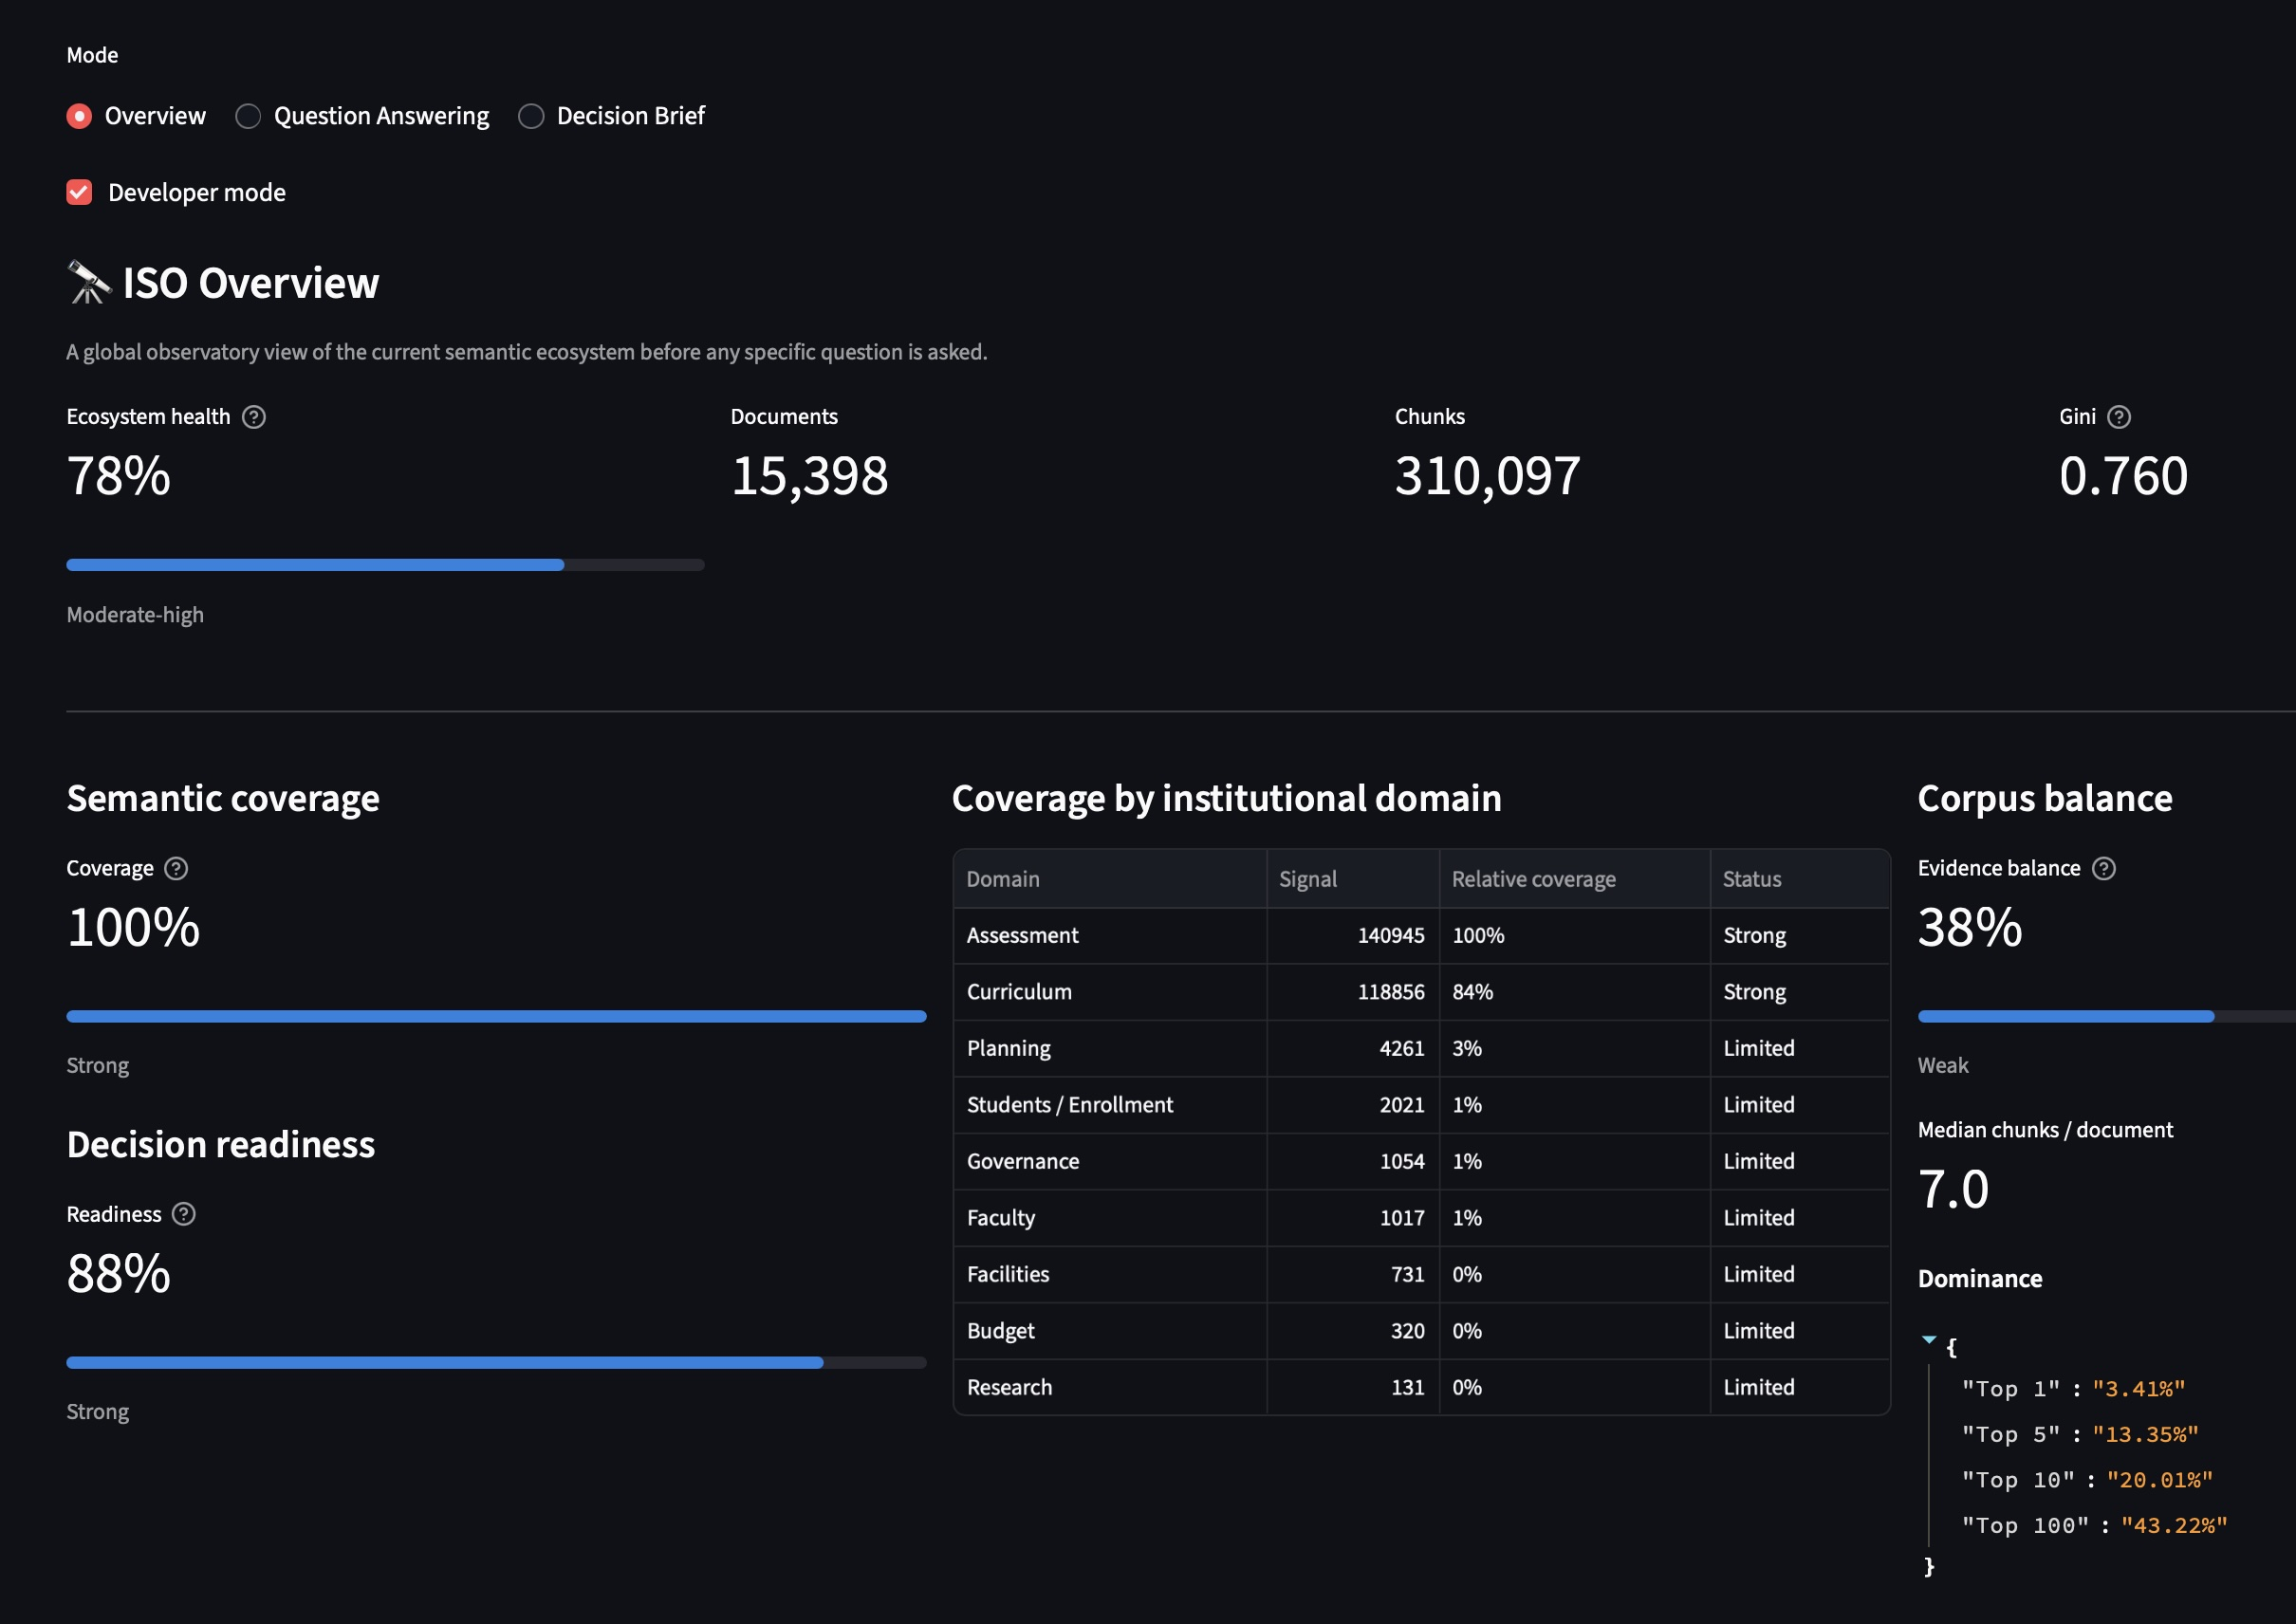
\includegraphics[width=0.95\textwidth]{semantic_observatory_health.jpg}
\end{center}

\vspace{2.3cm}
}
}

\end{columns}

\end{frame}

%=========================================================
\begin{frame}{Why Monitor Semantic Health?}

The quality of an AI system depends fundamentally on the quality
of the information ecosystem it reasons over.

\vspace{0.5cm}

\begin{block}{Example}

One corrupted spreadsheet generated nearly

\[
50,\!000
\]

semantic chunks.

Cleaning the spreadsheet reduced this to only a few hundred
chunks and improved the overall balance of the corpus.

\end{block}

\vspace{0.5cm}

The lesson is simple:

\vspace{0.1cm}

\Large

Healthy reasoning requires a healthy semantic ecosystem.

\end{frame}

%=========================================================
\begin{frame}{Semantic Health Metrics}

Current prototype corpus

\vspace{0.4cm}

\begin{table}

\begin{tabular}{lr}

\toprule

Documents & $\sim$15,400 \\

Semantic Chunks & $\sim$310,000 \\

Median Chunks / Document & 7 \\

90th Percentile & 24 \\

99th Percentile & 147 \\

Corpus Gini Coefficient & 0.76 \\

\bottomrule

\end{tabular}

\end{table}

\vspace{0.5cm}

The Gini coefficient provides a quantitative measure of whether
knowledge is reasonably distributed across the corpus or dominated
by only a handful of documents.

\end{frame}

%=========================================================
\begin{frame}{Developer Diagnostics}

Every question can be inspected in detail.

\vspace{0.4cm}

For every query we record

\begin{itemize}

\item FAISS retrieval

\item deduplication

\item reranking

\item thresholding

\item final evidence supplied to the LLM

\item execution timing

\end{itemize}

\vspace{0.5cm}

This transforms the retrieval pipeline from a "black box"
into an engineering system that can be measured, tested,
and improved.

\end{frame}

%=========================================================
\begin{frame}{The Working Prototype}

The current system already supports three distinct modes.

\vspace{0.5cm}

\begin{columns}

\column{0.31\textwidth}

\begin{block}{Question Answering}
Retrieve evidence and answer factual questions with citations.
\end{block}

\column{0.31\textwidth}

\begin{block}{Semantic Observatory}
Monitor the health, balance, and structure of the semantic ecosystem.
\end{block}

\column{0.31\textwidth}

\begin{block}{Decision Briefs}
Synthesize evidence across multiple domains for strategic questions.
\end{block}

\end{columns}

\vspace{0.7cm}

All three capabilities use the same underlying institutional knowledge layer.

\end{frame}

%=========================================================
\begin{frame}{Live Demonstration}

\Large

The demonstration will show three increasingly sophisticated uses.

\vspace{0.7cm}

\begin{enumerate}

\item \textbf{Question answering}

\smallskip

What is the CNU travel reimbursement policy?

\vspace{0.5cm}

\item \textbf{Semantic Health}

\smallskip

How do we know the information environment is reliable?

\vspace{0.5cm}

\item \textbf{Decision support}

\smallskip

What additional resources would be required to support a
Mechanical Engineering major?

\end{enumerate}

\end{frame}

%=========================================================
\begin{frame}{From Question Answering to Decision Support}

A factual question usually has a relatively direct answer.

\vspace{0.4cm}

\begin{block}{Question Answering}
What is the current travel reimbursement policy?
\end{block}

\vspace{0.5cm}

A strategic question requires synthesis across many sources.

\vspace{0.4cm}

\begin{block}{Decision Support}
What additional resources would be required to launch a
Mechanical Engineering major?
\end{block}

\vspace{0.5cm}

No single document contains the answer.

The answer emerges from the institutional knowledge ecosystem.

\end{frame}

%=========================================================
\begin{frame}{Mechanical Engineering Decision Brief}

The system decomposes the question into several evidence domains.

\vspace{0.4cm}

\begin{columns}

\column{0.48\textwidth}

\begin{itemize}
\item Existing faculty expertise
\item Required faculty expertise
\item Number of faculty lines
\item Existing curriculum
\item New course requirements
\end{itemize}

\column{0.48\textwidth}

\begin{itemize}
\item Laboratory space
\item Equipment needs
\item ABET requirements
\item Enrollment assumptions
\item Budget implications
\end{itemize}

\end{columns}

\vspace{0.6cm}

The resulting brief identifies evidence, likely gaps, risks,
uncertainties, and missing information.

\end{frame}

%=========================================================
\begin{frame}{What a Decision Brief Should Contain}

\begin{enumerate}

\item \textbf{Decision question}

\item \textbf{Executive summary}

\item \textbf{Relevant institutional evidence}

\item \textbf{Existing strengths}

\item \textbf{Resource gaps}

\item \textbf{Competing considerations}

\item \textbf{Risks and uncertainties}

\item \textbf{Missing information}

\item \textbf{Supporting sources}

\end{enumerate}

\vspace{0.5cm}

The system does not make the decision.

It structures the evidence needed for a defensible human decision.

\end{frame}

%=========================================================
\begin{frame}{Why This Is More Than a Chatbot}

\Large

\begin{block}{The language model is not the system.}

It is one reasoning service operating over carefully engineered
institutional knowledge.

\end{block}

\vspace{0.0cm}

The system also includes

\begin{itemize}
\item corpus stewardship,
\item provenance,
\item retrieval,
\item benchmarking,
\item observability,
\item validation,
\item and human governance.
\end{itemize}

\end{frame}

%=========================================================
\begin{frame}{What We Have Learned}

\small

\begin{block}{The hardest problem was not the language model.}

The most difficult and important work involved

\begin{itemize}
\setlength{\itemsep}{0.15cm}

\item determining what belongs in the corpus,

\item preserving provenance,

\item detecting corrupted, duplicated, or dominant documents,

\item measuring retrieval quality,

\item defining meaningful benchmarks,

\item and making the system observable.

\end{itemize}

\end{block}

\vspace{0.25cm}

\begin{center}
\large
Trustworthy AI depends upon trustworthy information infrastructure.
\end{center}

\end{frame}
%=========================================================
\begin{frame}{Prototype Status}

\small

The current prototype demonstrates that the architecture is practical
and technically feasible.

\vspace{0.25cm}

\begin{columns}[T]

\column{0.48\textwidth}

\begin{block}{Knowledge Infrastructure}

\begin{itemize}
\setlength{\itemsep}{0.08cm}
\item Document normalization
\item Semantic chunk generation
\item Semantic indexing
\item Semantic Observatory
\end{itemize}

\end{block}

\column{0.48\textwidth}

\begin{block}{Reasoning and Evaluation}

\begin{itemize}
\setlength{\itemsep}{0.08cm}
\item Retrieval benchmarking
\item Explainable diagnostics
\item Question answering
\item Decision Brief generation
\end{itemize}

\end{block}

\end{columns}

\vspace{0.3cm}

\begin{block}{Current transition}
The focus is shifting from proving technical feasibility toward
developing a sustained institutional decision-support capability.
\end{block}

\end{frame}

%=========================================================
\begin{frame}{The Road Ahead}

\begin{center}

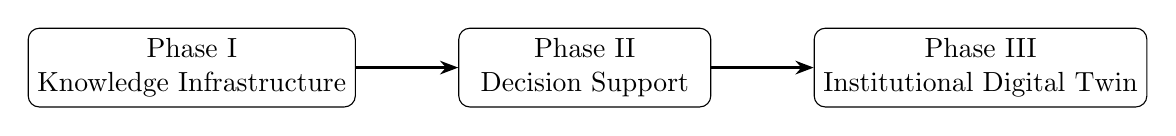
\begin{tikzpicture}[
node distance=1.3cm,
>=Stealth,
every node/.style={
draw,
rounded corners,
minimum width=3.2cm,
minimum height=1cm,
align=center}
]

\node (phase1) {Phase I\\Knowledge Infrastructure};

\node (phase2) [right=of phase1] {Phase II\\Decision Support};

\node (phase3) [right=of phase2] {Phase III\\Institutional Digital Twin};

\draw[->,thick] (phase1)--(phase2);
\draw[->,thick] (phase2)--(phase3);

\end{tikzpicture}

\end{center}

\vspace{0.8cm}

Today's prototype completes much of the first phase and begins
to demonstrate the second.

\end{frame}

%=========================================================
\begin{frame}{Near-Term Opportunities}

Examples that could be explored during the coming months include

\vspace{0.5cm}

\begin{itemize}

\item Mechanical Engineering program planning

\item Faculty hiring scenarios

\item Enrollment forecasting

\item Space utilization

\item Laboratory planning

\item Accreditation support

\item Strategic budgeting

\item Institutional policy analysis

\end{itemize}

\vspace{0.5cm}

The same semantic infrastructure supports each of these applications.

\end{frame}

%=========================================================
\begin{frame}{An Emerging View of AI}

One lesson has become increasingly clear during development.

\vspace{0.6cm}

\begin{block}{Traditional View}

AI is a model that answers questions.

\end{block}

\vspace{0.5cm}

\begin{block}{Our Working View}

AI is one reasoning component operating within a carefully
engineered information ecosystem.

\end{block}

\vspace{0.6cm}

The quality of reasoning is often limited more by the quality
of the semantic ecosystem than by the reasoning model itself.

\end{frame}

%=========================================================
\begin{frame}{Digital Twin}

A long-term objective is to develop a semantic representation
of the institution itself.

\vspace{0.5cm}

Rather than storing only documents,

the system gradually develops an interconnected representation of

\vspace{0.4cm}

\begin{itemize}

\item people

\item programs

\item curricula

\item facilities

\item policies

\item finances

\item strategic initiatives

\item institutional relationships

\end{itemize}

\vspace{0.2cm}

This evolving semantic model provides the foundation for
institutional reasoning.

\end{frame}

%=========================================================
\begin{frame}{One Observation}

During development we discovered something unexpected.

\vspace{0.7cm}

\begin{center}

\Large

The engineering required to create trustworthy institutional
knowledge turned out to be substantially more difficult than
connecting a language model.

\end{center}

\vspace{0.8cm}

This project has therefore become as much about
\textbf{knowledge engineering}
as it is about artificial intelligence.

\end{frame}

%=========================================================
\begin{frame}{Conclusions}

\begin{itemize}

\item Explainable AI for higher education is achievable.

\bigskip

\item Institutional knowledge can be organized into a reusable
semantic infrastructure.

\bigskip

\item Trust depends upon explainability, provenance,
and continuous measurement.

\bigskip

\item A healthy semantic ecosystem is essential for
trustworthy institutional reasoning.

\end{itemize}

\end{frame}

%=========================================================

%=========================================================
\begin{frame}

\centering

\vspace{0.8cm}

{\LARGE
The objective is not to automate\\[0.3cm]
university decision making.
}

\vspace{1.2cm}

{\Large
The objective is to help people make
better-informed,
more transparent,
and more defensible decisions.
}

\vfill

{\large
Thank you.
}

\end{frame}

%=========================================================
\end{document}